本机按冻结协议登记了 1920 项正式任务，全部结束，其中 0 项未返回满足输出标准的正常样本。失败计数与原始输出均保留；该总任务数包含配对执行，并非 1920 个独立模型。每个模型、预算及工作流的独立重复数为 24。

正常输出中，独立核验记录的最大数值路径差为 $2.36\times10^{-8}$，接受事件失配总数为 0。这一陈述以数值核验及当前目标库为边界，不构成一般轨迹或平稳分布证明。

quasi-DEER MALA 的模型—预算组中位缓存执行速度比范围为 0.0192 至 0.174，研究审计工作流速度比范围为 0.0715 至 0.739。速度比定义为同核顺序时间除以并行时间，小于 1 表示并行执行更慢；这里只统计成对有效输出，失败另行报告。

Online Picard RWM 的模型—预算组中位缓存执行速度比范围为 0.0503 至 0.809，研究审计工作流速度比范围为 0.226 至 0.814。速度比定义为同核顺序时间除以并行时间，小于 1 表示并行执行更慢；这里只统计成对有效输出，失败另行报告。

\begin{figure}[htbp]\centering
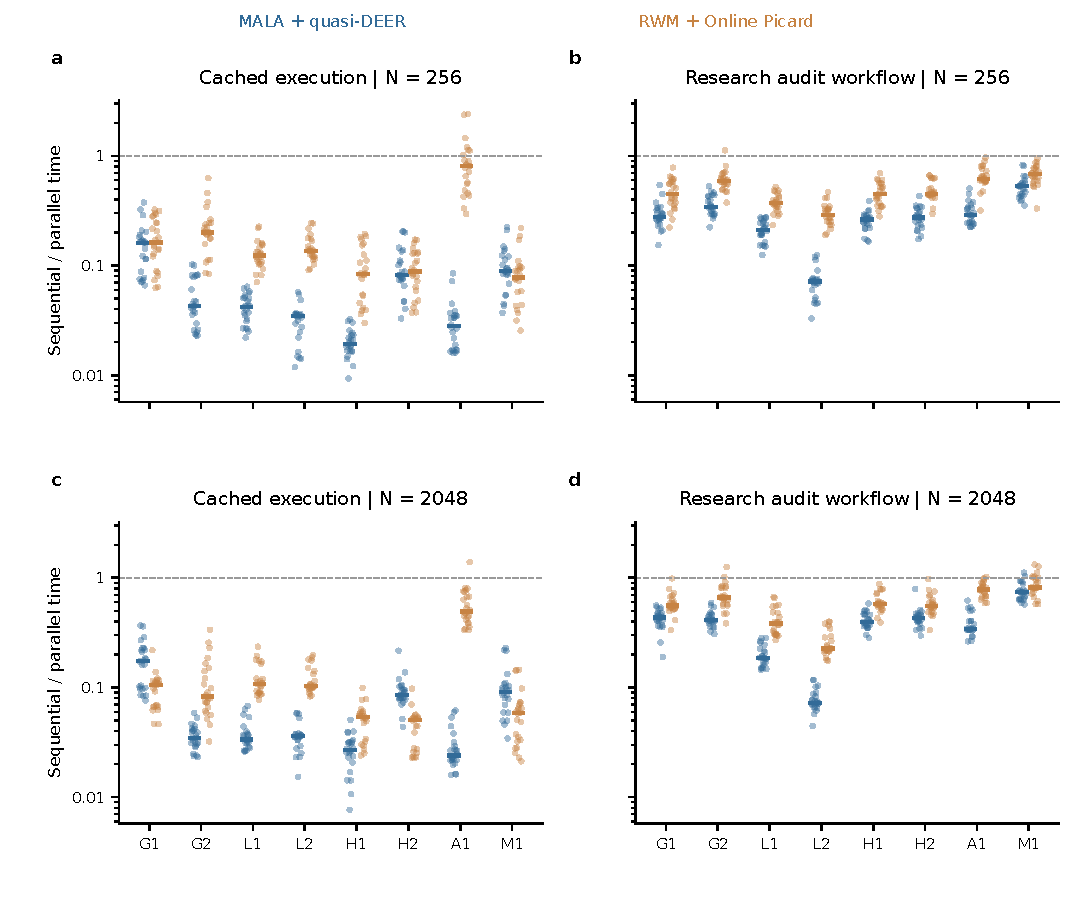
\includegraphics[width=\linewidth]{../../figures/software/paired-costs.pdf}
\caption{同核成对成本。上、下行分别为每链保留256和2048步；左列为两次缓存重放时间的中位数之比，右列为含编译、预热/丢弃段和独立核验的工作流时间比。每个点为一个独立重复中的配对比，短线为组中位数；同一轨迹的计时重放不当作统计重复。虚线表示速度比1。任何缺失配对均在原始任务及失败表中保留。}
\end{figure}

表中列出较大预算下的函数最大平方误差。L1/L2 采用有限参考，因此相应数值是参考平方差。完整逐函数误差、逐点区间、参考敏感性区间、失败比例区间及两预算结果随机器可读材料交付。不能把表中的最小数值自动解释为确定排名。

\begin{table}[htbp]\centering\small\setlength{\tabcolsep}{3pt}\begin{tabular}{lrrrrr}\toprule

目标 & 顺序MALA & quasi-DEER & 顺序RWM & Picard & NUTS\\\midrule

G1 & $0.00199$ (0) & $0.00199$ (0) & $0.00542$ (0) & $0.00542$ (0) & $0.000531$ (0)\\

G2 & $0.125$ (0) & $0.125$ (0) & $0.164$ (0) & $0.164$ (0) & $0.000322$ (0)\\

L1 & $0.000255$ (0) & $0.000255$ (0) & $0.000673$ (0) & $0.000673$ (0) & $1.46\times10^{-5}$ (0)\\

L2 & $6.22\times10^{-6}$ $\dagger$ (0) & $6.22\times10^{-6}$ $\dagger$ (0) & $1.91\times10^{-5}$ $\dagger$ (0) & $1.91\times10^{-5}$ $\dagger$ (0) & $2.28\times10^{-7}$ $\dagger$ (0)\\

H1 & $0.138$ (0) & $0.138$ (0) & $0.131$ (0) & $0.131$ (0) & $0.112$ (0)\\

H2 & $0.0215$ (0) & $0.0215$ (0) & $0.0376$ (0) & $0.0376$ (0) & $6.11\times10^{-5}$ (0)\\

A1 & $0.00803$ (0) & $0.00803$ (0) & $0.856$ (0) & $0.856$ (0) & $0.000665$ (0)\\

M1 & $0.252$ (0) & $0.252$ (0) & $0.359$ (0) & $0.359$ (0) & $0.296$ (0)\\

\bottomrule\end{tabular}\caption{每链保留2048步时的最大函数平方误差/参考平方差。括号内为该组24次重复中的输出失败数；有失败时，误差仅描述成功输出。误差不包含失败的假定损失，不代表无条件达标。$\dagger$表示参考精度未确定，该行仅展示参考平方差，不能判断全函数精度达标。}\end{table}

按前述工作流口径汇总，正式尝试合计耗时 5080.9 秒，其中失败任务耗时 0.0 秒。另有缓存计时重放开销5711.5秒，完整保留但不重复计入单次工作流成本。逐组成本及全部失败分母另存分析结果。

NUTS 在 46 个已返回有限样本的任务中记录到发散，总计 2358 个保留转移的发散事件。发散与数值输出失败分别呈现，不能因为数组有限而删除这一诊断。多峰和漏斗目标上的误差须结合模式占比及尺度函数理解。

NUTS另有6861个保留转移达到255个积分步的设定上限；积分步数及逐次适配参数随原始记录保存。

采样接口期间记录的逐任务进程RSS峰值范围为244.3至549.0 MiB；它包含进程已驻留内存，只覆盖接口调用阶段，不能解释为每种算法的独占增量内存或整项任务的严格峰值。

quasi-DEER的模型—预算组中，单个输出转移对应的前向转移映射求值次数中位数范围为14.58至66.15，顺序MH为1。

Online Picard的模型—预算组中，单个输出转移对应的前向转移映射求值次数中位数范围为2.00至21.38，顺序MH为1。

这些程序层面的映射调用计数包含丢弃段和拒绝自环，尚不包含独立审计；它们不是浮点运算量或密度/梯度调用次数。quasi-DEER的JVP另存，因此不能仅据调用数精确分解运行瓶颈。

\begin{figure}[htbp]\centering
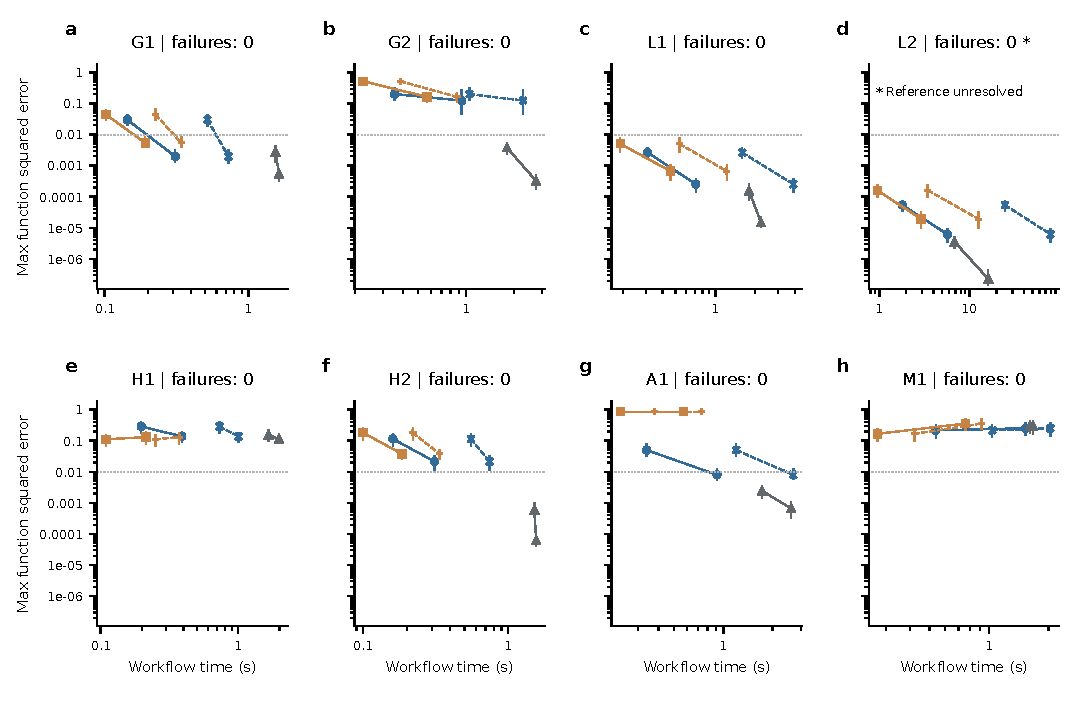
\includegraphics[width=\linewidth]{../../figures/software/error-cost.pdf}
\caption{固定采样计划的误差—成本关系。横轴为成功输出条件下的工作流时间中位数，全部尝试和失败成本另表保存。每条线连接同一指定工作流的两个预算点，不表示中间预算已被测量。蓝色为MALA、橙色为RWM、灰色为NUTS；实线/圆或方形为顺序MH，虚线/叉号为相应时间执行器，三角形为NUTS。误差取预声明函数中最大的重复平均平方误差；L1/L2为有限参考平方差。线段区间为逐点95\%重复重采样区间，有限参考的共同误差敏感性另行传播；传播采用正态对角协方差工作假设，非同时保证。星号表示参考精度未确定，该面板仅供探索性平方差比较。面板标题列出该模型全部正式任务中的输出失败数，失败组的误差为条件结果。点虚线标出0.01作为预声明误差阈值。}
\end{figure}

\noindent mala/sequential在较长预算、$\epsilon=0.1$下的逐点判断为：区间低于阈值2个目标，区间高于阈值4个，跨阈值1个，参考或输出条件不足1个。\par

\noindent mala/quasi\_deer在较长预算、$\epsilon=0.1$下的逐点判断为：区间低于阈值2个目标，区间高于阈值4个，跨阈值1个，参考或输出条件不足1个。\par

\noindent rwm/sequential在较长预算、$\epsilon=0.1$下的逐点判断为：区间低于阈值2个目标，区间高于阈值5个，跨阈值0个，参考或输出条件不足1个。\par

\noindent rwm/online\_picard在较长预算、$\epsilon=0.1$下的逐点判断为：区间低于阈值2个目标，区间高于阈值5个，跨阈值0个，参考或输出条件不足1个。\par

\noindent nuts/sequential在较长预算、$\epsilon=0.1$下的逐点判断为：区间低于阈值5个目标，区间高于阈值2个，跨阈值0个，参考或输出条件不足1个。\par

这些判断仅对应两个已测量预算中的较长预算，不构成同时置信结论，也不提供单次运行可观测的停止规则或精确的达标时间。

正式生成式检查完成64个新数据集、五种工作流，共320次拟合，其中0次输出失败。90\%后验区间的覆盖估计及其二项区间按数据集作为独立单位报告；保留所有秩与原始样本。抽稀秩仍可能相关，这一检查不提供一般SBC一致性证明。

\noindent mala/sequential：覆盖率 0.844，95\%二项区间 [0.731, 0.922]。\par

\noindent mala/quasi\_deer：覆盖率 0.844，95\%二项区间 [0.731, 0.922]。\par

\noindent rwm/sequential：覆盖率 0.828，95\%二项区间 [0.713, 0.911]。\par

\noindent rwm/online\_picard：覆盖率 0.828，95\%二项区间 [0.713, 0.911]。\par

\noindent nuts/sequential：覆盖率 0.828，95\%二项区间 [0.713, 0.911]。\par

正式生成式检查另记录到0个保留转移的发散事件，涉及0次拟合；该诊断与输出失败分开保存。

本次覆盖率点估计均低于名义90\%，而相应二项区间均包含90\%。这一有限重复结果既不能证明完全校准，也不应被改写为已确证系统性覆盖不足。

对数似然测试量也完成320次拟合的伴随分析，共记录0个秩并列。逐方法秩直方图、抽稀后相关性及解析期望误差随原始数据交付；这些描述性诊断不构成统一性检验或正确性证书。

L2 的参考符号事件在262144个相关样本中均为零，Rhat 对该函数不可判定，不能把零经验方差当作事件概率已被精确确定。因此保留原函数集合，并将L2全函数精度判定标记为未确定。没有通过删除该函数得到达标结论。

上述结果来自历史Mac CPU协议，不包含后续Windows实验；原生Windows实现及其独立协议的实测结果在后文另行报告。
